% !TeX root = ../../../main.tex

%\tikzexternaldisable%

\newcommand{\tikzmark}[2]{\tikz[overlay, remember picture,
	baseline=(#1.base), font=\tiny] \node (#1) {#2};}%

\begin{minipage}[t][3cm][b]{.2\textwidth}%
	\topskip0pt%
	\rightskip0pt%
	\leftskip0pt%
		\hspace{-0.2cm}%
		\resizebox{\linewidth}{3cm}{%
		\trimbox{0.2cm 0.22cm 0.3cm 0.12cm}{ %
		% !TeX root = ../../../main.tex

% This file was created by matlab2tikz.
%
%The latest updates can be retrieved from
%  http://www.mathworks.com/matlabcentral/fileexchange/22022-matlab2tikz-matlab2tikz
%where you can also make suggestions and rate matlab2tikz.
%
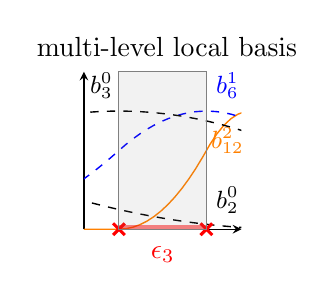
\begin{tikzpicture}[remember picture]
\def\lineWidth{0.5pt}
\def\knotWidth{1.1pt}
\def\knotSize{3pt}
\def\elementWidth{3pt}
\def\colorLevelOne{black}
\def\colorLevelTwo{blue}
\def\colorLevelThree{orange}
\tikzset{% 
	elementLineStyle/.style={%
		color=red,solid,line width=\elementWidth, opacity=0.5
	}
}

\tikzset{% 
	knotsStyle/.style={%
		color=red,line width=\knotWidth,mark size=\knotSize,only marks,mark=x,mark options={solid}
	}
}

\tikzset{% 
	inactive/.style={%
		color=white!85!black,solid,line width=\lineWidth
	}
}

\tikzset{% 
	ap/.style={%
		dashed,line width=\lineWidth
	}
}

\tikzset{% 
	am/.style={%
		white!70!black,densely dotted,line width=\lineWidth
	}
}


\tikzset{% 
	aa/.style={%
		solid,line width=\lineWidth
	}
}

\begin{axis}[%
width=2cm,
height=2cm,
scale only axis,
xmin=0.20,
xmax=0.425,
ymin=0,
ymax=1,
axis background/.style={draw=none},
ymajorgrids=false,
%
axis y line=left,
axis x line=bottom,
%footnotesize,
ytick={0,1},
%xtick={0.25,0.375},
ticks=none,
tickpos=left,
ytick align=outside,
xtick align=outside,
tick label style ={font=\small},
label style ={font=\small},
legend style={ font =\small },
]
\addplot [color=\colorLevelThree,aa]
table[row sep=crcr]{%
	-1	0\\
	-0.99	0\\
	-0.98	0\\
	-0.97	0\\
	-0.96	0\\
	-0.95	0\\
	-0.94	0\\
	-0.93	0\\
	-0.92	0\\
	-0.91	0\\
	-0.9	0\\
	-0.89	0\\
	-0.88	0\\
	-0.87	0\\
	-0.86	0\\
	-0.85	0\\
	-0.84	0\\
	-0.83	0\\
	-0.82	0\\
	-0.81	0\\
	-0.8	0\\
	-0.79	0\\
	-0.78	0\\
	-0.77	0\\
	-0.76	0\\
	-0.75	0\\
	-0.74	0\\
	-0.73	0\\
	-0.72	0\\
	-0.71	0\\
	-0.7	0\\
	-0.69	0\\
	-0.68	0\\
	-0.67	0\\
	-0.66	0\\
	-0.65	0\\
	-0.64	0\\
	-0.63	0\\
	-0.62	0\\
	-0.61	0\\
	-0.6	0\\
	-0.59	0\\
	-0.58	0\\
	-0.57	0\\
	-0.56	0\\
	-0.55	0\\
	-0.54	0\\
	-0.53	0\\
	-0.52	0\\
	-0.51	0\\
	-0.5	0\\
	-0.49	0\\
	-0.48	0\\
	-0.47	0\\
	-0.46	0\\
	-0.45	0\\
	-0.44	0\\
	-0.43	0\\
	-0.42	0\\
	-0.41	0\\
	-0.4	0\\
	-0.39	0\\
	-0.38	0\\
	-0.37	0\\
	-0.36	0\\
	-0.35	0\\
	-0.34	0\\
	-0.33	0\\
	-0.32	0\\
	-0.31	0\\
	-0.3	0\\
	-0.29	0\\
	-0.28	0\\
	-0.27	0\\
	-0.26	0\\
	-0.25	0\\
	-0.24	0\\
	-0.23	0\\
	-0.22	0\\
	-0.21	0\\
	-0.2	0\\
	-0.19	0\\
	-0.18	0\\
	-0.17	0\\
	-0.16	0\\
	-0.15	0\\
	-0.14	0\\
	-0.13	0\\
	-0.12	0\\
	-0.11	0\\
	-0.1	0\\
	-0.09	0\\
	-0.08	0\\
	-0.07	0\\
	-0.0599999999999999	0\\
	-0.0499999999999999	0\\
	-0.04	0\\
	-0.03	0\\
	-0.02	0\\
	-0.01	0\\
	0	0\\
	0.01	0\\
	0.02	0\\
	0.03	0\\
	0.04	0\\
	0.0499999999999999	0\\
	0.0599999999999999	0\\
	0.07	0\\
	0.08	0\\
	0.09	0\\
	0.1	0\\
	0.11	0\\
	0.12	0\\
	0.13	0\\
	0.14	0\\
	0.15	0\\
	0.16	0\\
	0.17	0\\
	0.18	0\\
	0.19	0\\
	0.2	0\\
	0.21	0\\
	0.22	0\\
	0.23	0\\
	0.24	0\\
	0.25	0\\
	0.26	0.00320000000000001\\
	0.27	0.0128\\
	0.28	0.0288000000000001\\
	0.29	0.0512000000000001\\
	0.3	0.0799999999999998\\
	0.31	0.1152\\
	0.32	0.1568\\
	0.33	0.2048\\
	0.34	0.2592\\
	0.35	0.32\\
	0.36	0.3872\\
	0.37	0.4608\\
	0.38	0.5384\\
	0.39	0.6056\\
	0.4	0.66\\
	0.41	0.7016\\
	0.42	0.7304\\
	0.43	0.7464\\
	0.44	0.7496\\
	0.45	0.74\\
	0.46	0.7176\\
	0.47	0.6824\\
	0.48	0.6344\\
	0.49	0.5736\\
	0.5	0.5\\
	0.51	0.4232\\
	0.52	0.3528\\
	0.53	0.2888\\
	0.54	0.2312\\
	0.55	0.18\\
	0.56	0.1352\\
	0.57	0.0967999999999998\\
	0.58	0.0647999999999998\\
	0.59	0.0392000000000001\\
	0.6	0.02\\
	0.61	0.00720000000000001\\
	0.62	0.000800000000000001\\
	0.63	0\\
	0.64	0\\
	0.65	0\\
	0.66	0\\
	0.67	0\\
	0.68	0\\
	0.69	0\\
	0.7	0\\
	0.71	0\\
	0.72	0\\
	0.73	0\\
	0.74	0\\
	0.75	0\\
	0.76	0\\
	0.77	0\\
	0.78	0\\
	0.79	0\\
	0.8	0\\
	0.81	0\\
	0.82	0\\
	0.83	0\\
	0.84	0\\
	0.85	0\\
	0.86	0\\
	0.87	0\\
	0.88	0\\
	0.89	0\\
	0.9	0\\
	0.91	0\\
	0.92	0\\
	0.93	0\\
	0.94	0\\
	0.95	0\\
	0.96	0\\
	0.97	0\\
	0.98	0\\
	0.99	0\\
	1	0\\
};
\addplot [color=\colorLevelTwo,ap]
table[row sep=crcr]{%
	0	0\\
	0.01	0.000800000000000001\\
	0.02	0.00320000000000001\\
	0.03	0.00720000000000001\\
	0.04	0.0128\\
	0.0499999999999999	0.0199999999999999\\
	0.0599999999999999	0.0287999999999999\\
	0.07	0.0391999999999999\\
	0.08	0.0511999999999999\\
	0.09	0.0648\\
	0.1	0.08\\
	0.11	0.0968\\
	0.12	0.1152\\
	0.13	0.1352\\
	0.14	0.1568\\
	0.15	0.18\\
	0.16	0.2048\\
	0.17	0.2312\\
	0.18	0.2592\\
	0.19	0.2888\\
	0.2	0.32\\
	0.21	0.3528\\
	0.22	0.3872\\
	0.23	0.4232\\
	0.24	0.4608\\
	0.25	0.5\\
	0.26	0.5384\\
	0.27	0.5736\\
	0.28	0.6056\\
	0.29	0.6344\\
	0.3	0.66\\
	0.31	0.6824\\
	0.32	0.7016\\
	0.33	0.7176\\
	0.34	0.7304\\
	0.35	0.74\\
	0.36	0.7464\\
	0.37	0.7496\\
	0.38	0.7496\\
	0.39	0.7464\\
	0.4	0.74\\
	0.41	0.7304\\
	0.42	0.7176\\
	0.43	0.7016\\
	0.44	0.6824\\
	0.45	0.66\\
	0.46	0.6344\\
	0.47	0.6056\\
	0.48	0.5736\\
	0.49	0.5384\\
	0.5	0.5\\
	0.51	0.4608\\
	0.52	0.4232\\
	0.53	0.3872\\
	0.54	0.3528\\
	0.55	0.32\\
	0.56	0.2888\\
	0.57	0.2592\\
	0.58	0.2312\\
	0.59	0.2048\\
	0.6	0.18\\
	0.61	0.1568\\
	0.62	0.1352\\
	0.63	0.1152\\
	0.64	0.0968\\
	0.65	0.0800000000000001\\
	0.66	0.0648000000000001\\
	0.67	0.0512000000000001\\
	0.68	0.0392000000000001\\
	0.69	0.0288000000000001\\
	0.7	0.02\\
	0.71	0.0128\\
	0.72	0.00720000000000001\\
	0.73	0.00320000000000001\\
	0.74	0.000800000000000001\\
	0.75	0\\
};

\addplot [color=\colorLevelOne,ap]
table[row sep=crcr]{%
	-1	0\\
	-0.995	5.00000000000001e-05\\
	-0.99	0.0002\\
	-0.985	0.000450000000000001\\
	-0.98	0.000800000000000001\\
	-0.975	0.00125\\
	-0.97	0.0018\\
	-0.965	0.00245\\
	-0.96	0.00320000000000001\\
	-0.955	0.00405000000000001\\
	-0.95	0.00500000000000001\\
	-0.945	0.00605000000000001\\
	-0.94	0.00720000000000001\\
	-0.935	0.00844999999999999\\
	-0.93	0.00980000000000002\\
	-0.925	0.01125\\
	-0.92	0.0128\\
	-0.915	0.01445\\
	-0.91	0.0162\\
	-0.905	0.01805\\
	-0.9	0.02\\
	-0.895	0.02205\\
	-0.89	0.0242\\
	-0.885	0.02645\\
	-0.88	0.0288\\
	-0.875	0.03125\\
	-0.87	0.0338\\
	-0.865	0.03645\\
	-0.86	0.0392\\
	-0.855	0.04205\\
	-0.85	0.045\\
	-0.845	0.04805\\
	-0.84	0.0512\\
	-0.835	0.05445\\
	-0.83	0.0578\\
	-0.825	0.06125\\
	-0.82	0.0648\\
	-0.815	0.06845\\
	-0.81	0.0722\\
	-0.805	0.07605\\
	-0.8	0.08\\
	-0.795	0.0840500000000001\\
	-0.79	0.0882\\
	-0.785	0.09245\\
	-0.78	0.0968\\
	-0.775	0.10125\\
	-0.77	0.1058\\
	-0.765	0.11045\\
	-0.76	0.1152\\
	-0.755	0.12005\\
	-0.75	0.125\\
	-0.745	0.13005\\
	-0.74	0.1352\\
	-0.735	0.14045\\
	-0.73	0.1458\\
	-0.725	0.15125\\
	-0.72	0.1568\\
	-0.715	0.16245\\
	-0.71	0.1682\\
	-0.705	0.17405\\
	-0.7	0.18\\
	-0.695	0.18605\\
	-0.69	0.1922\\
	-0.685	0.19845\\
	-0.68	0.2048\\
	-0.675	0.21125\\
	-0.67	0.2178\\
	-0.665	0.22445\\
	-0.66	0.2312\\
	-0.655	0.23805\\
	-0.65	0.245\\
	-0.645	0.25205\\
	-0.64	0.2592\\
	-0.635	0.26645\\
	-0.63	0.2738\\
	-0.625	0.28125\\
	-0.62	0.2888\\
	-0.615	0.29645\\
	-0.61	0.3042\\
	-0.605	0.31205\\
	-0.6	0.32\\
	-0.595	0.32805\\
	-0.59	0.3362\\
	-0.585	0.34445\\
	-0.58	0.3528\\
	-0.575	0.36125\\
	-0.57	0.3698\\
	-0.565	0.37845\\
	-0.56	0.3872\\
	-0.555	0.39605\\
	-0.55	0.405\\
	-0.545	0.41405\\
	-0.54	0.4232\\
	-0.535	0.43245\\
	-0.53	0.4418\\
	-0.525	0.45125\\
	-0.52	0.4608\\
	-0.515	0.47045\\
	-0.51	0.4802\\
	-0.505	0.49005\\
	-0.5	0.5\\
	-0.495	0.5099\\
	-0.49	0.5196\\
	-0.485	0.5291\\
	-0.48	0.5384\\
	-0.475	0.5475\\
	-0.47	0.5564\\
	-0.465	0.5651\\
	-0.46	0.5736\\
	-0.455	0.5819\\
	-0.45	0.59\\
	-0.445	0.5979\\
	-0.44	0.6056\\
	-0.435	0.6131\\
	-0.43	0.6204\\
	-0.425	0.6275\\
	-0.42	0.6344\\
	-0.415	0.6411\\
	-0.41	0.6476\\
	-0.405	0.6539\\
	-0.4	0.66\\
	-0.395	0.6659\\
	-0.39	0.6716\\
	-0.385	0.6771\\
	-0.38	0.6824\\
	-0.375	0.6875\\
	-0.37	0.6924\\
	-0.365	0.6971\\
	-0.36	0.7016\\
	-0.355	0.7059\\
	-0.35	0.71\\
	-0.345	0.7139\\
	-0.34	0.7176\\
	-0.335	0.7211\\
	-0.33	0.7244\\
	-0.325	0.7275\\
	-0.32	0.7304\\
	-0.315	0.7331\\
	-0.31	0.7356\\
	-0.305	0.7379\\
	-0.3	0.74\\
	-0.295	0.7419\\
	-0.29	0.7436\\
	-0.285	0.7451\\
	-0.28	0.7464\\
	-0.275	0.7475\\
	-0.27	0.7484\\
	-0.265	0.7491\\
	-0.26	0.7496\\
	-0.255	0.7499\\
	-0.25	0.75\\
	-0.245	0.7499\\
	-0.24	0.7496\\
	-0.235	0.7491\\
	-0.23	0.7484\\
	-0.225	0.7475\\
	-0.22	0.7464\\
	-0.215	0.7451\\
	-0.21	0.7436\\
	-0.205	0.7419\\
	-0.2	0.74\\
	-0.195	0.7379\\
	-0.19	0.7356\\
	-0.185	0.7331\\
	-0.18	0.7304\\
	-0.175	0.7275\\
	-0.17	0.7244\\
	-0.165	0.7211\\
	-0.16	0.7176\\
	-0.155	0.7139\\
	-0.15	0.71\\
	-0.145	0.7059\\
	-0.14	0.7016\\
	-0.135	0.6971\\
	-0.13	0.6924\\
	-0.125	0.6875\\
	-0.12	0.6824\\
	-0.115	0.6771\\
	-0.11	0.6716\\
	-0.105	0.6659\\
	-0.1	0.66\\
	-0.095	0.6539\\
	-0.09	0.6476\\
	-0.085	0.6411\\
	-0.08	0.6344\\
	-0.075	0.6275\\
	-0.07	0.6204\\
	-0.0649999999999999	0.6131\\
	-0.0599999999999999	0.6056\\
	-0.0549999999999999	0.5979\\
	-0.0499999999999999	0.59\\
	-0.0449999999999999	0.5819\\
	-0.04	0.5736\\
	-0.035	0.5651\\
	-0.03	0.5564\\
	-0.025	0.5475\\
	-0.02	0.5384\\
	-0.015	0.5291\\
	-0.01	0.5196\\
	-0.005	0.5099\\
	0	0.5\\
	0.005	0.49005\\
	0.01	0.4802\\
	0.015	0.47045\\
	0.02	0.4608\\
	0.025	0.45125\\
	0.03	0.4418\\
	0.035	0.43245\\
	0.04	0.4232\\
	0.0449999999999999	0.41405\\
	0.0499999999999999	0.405\\
	0.0549999999999999	0.39605\\
	0.0599999999999999	0.3872\\
	0.0649999999999999	0.37845\\
	0.07	0.3698\\
	0.075	0.36125\\
	0.08	0.3528\\
	0.085	0.34445\\
	0.09	0.3362\\
	0.095	0.32805\\
	0.1	0.32\\
	0.105	0.31205\\
	0.11	0.3042\\
	0.115	0.29645\\
	0.12	0.2888\\
	0.125	0.28125\\
	0.13	0.2738\\
	0.135	0.26645\\
	0.14	0.2592\\
	0.145	0.25205\\
	0.15	0.245\\
	0.155	0.23805\\
	0.16	0.2312\\
	0.165	0.22445\\
	0.17	0.2178\\
	0.175	0.21125\\
	0.18	0.2048\\
	0.185	0.19845\\
	0.19	0.1922\\
	0.195	0.18605\\
	0.2	0.18\\
	0.205	0.17405\\
	0.21	0.1682\\
	0.215	0.16245\\
	0.22	0.1568\\
	0.225	0.15125\\
	0.23	0.1458\\
	0.235	0.14045\\
	0.24	0.1352\\
	0.245	0.13005\\
	0.25	0.125\\
	0.255	0.12005\\
	0.26	0.1152\\
	0.265	0.11045\\
	0.27	0.1058\\
	0.275	0.10125\\
	0.28	0.0968\\
	0.285	0.09245\\
	0.29	0.0882\\
	0.295	0.08405\\
	0.3	0.08\\
	0.305	0.07605\\
	0.31	0.0722\\
	0.315	0.06845\\
	0.32	0.0648\\
	0.325	0.06125\\
	0.33	0.0578\\
	0.335	0.05445\\
	0.34	0.0512\\
	0.345	0.04805\\
	0.35	0.045\\
	0.355	0.04205\\
	0.36	0.0392\\
	0.365	0.03645\\
	0.37	0.0338\\
	0.375	0.03125\\
	0.38	0.0288\\
	0.385	0.02645\\
	0.39	0.0242\\
	0.395	0.02205\\
	0.4	0.02\\
	0.405	0.01805\\
	0.41	0.0162\\
	0.415	0.01445\\
	0.42	0.0128\\
	0.425	0.01125\\
	0.43	0.00980000000000002\\
	0.435	0.00845000000000001\\
	0.44	0.00720000000000001\\
	0.445	0.00605000000000001\\
	0.45	0.00500000000000001\\
	0.455	0.00405000000000001\\
	0.46	0.00320000000000001\\
	0.465	0.00245\\
	0.47	0.0018\\
	0.475	0.00125\\
	0.48	0.000800000000000001\\
	0.485	0.000450000000000001\\
	0.49	0.0002\\
	0.495	5.00000000000001e-05\\
	0.5	0\\
	0.505	0\\
	0.51	0\\
	0.515	0\\
	0.52	0\\
	0.525	0\\
	0.53	0\\
	0.535	0\\
	0.54	0\\
	0.545	0\\
	0.55	0\\
	0.555	0\\
	0.56	0\\
	0.565	0\\
	0.57	0\\
	0.575	0\\
	0.58	0\\
	0.585	0\\
	0.59	0\\
	0.595	0\\
	0.6	0\\
	0.605	0\\
	0.61	0\\
	0.615	0\\
	0.62	0\\
	0.625	0\\
	0.63	0\\
	0.635	0\\
	0.64	0\\
	0.645	0\\
	0.65	0\\
	0.655	0\\
	0.66	0\\
	0.665	0\\
	0.67	0\\
	0.675	0\\
	0.68	0\\
	0.685	0\\
	0.69	0\\
	0.695	0\\
	0.7	0\\
	0.705	0\\
	0.71	0\\
	0.715	0\\
	0.72	0\\
	0.725	0\\
	0.73	0\\
	0.735	0\\
	0.74	0\\
	0.745	0\\
	0.75	0\\
	0.755	0\\
	0.76	0\\
	0.765	0\\
	0.77	0\\
	0.775	0\\
	0.78	0\\
	0.785	0\\
	0.79	0\\
	0.795	0\\
	0.8	0\\
	0.805	0\\
	0.81	0\\
	0.815	0\\
	0.82	0\\
	0.825	0\\
	0.83	0\\
	0.835	0\\
	0.84	0\\
	0.845	0\\
	0.85	0\\
	0.855	0\\
	0.86	0\\
	0.865	0\\
	0.87	0\\
	0.875	0\\
	0.88	0\\
	0.885	0\\
	0.89	0\\
	0.895	0\\
	0.9	0\\
	0.905	0\\
	0.91	0\\
	0.915	0\\
	0.92	0\\
	0.925	0\\
	0.93	0\\
	0.935	0\\
	0.94	0\\
	0.945	0\\
	0.95	0\\
	0.955	0\\
	0.96	0\\
	0.965	0\\
	0.97	0\\
	0.975	0\\
	0.98	0\\
	0.985	0\\
	0.99	0\\
	0.995	0\\
	1	0\\
};
\addplot [color=\colorLevelOne,ap]
table[row sep=crcr]{%
	-1	0\\
	-0.995	0\\
	-0.99	0\\
	-0.985	0\\
	-0.98	0\\
	-0.975	0\\
	-0.97	0\\
	-0.965	0\\
	-0.96	0\\
	-0.955	0\\
	-0.95	0\\
	-0.945	0\\
	-0.94	0\\
	-0.935	0\\
	-0.93	0\\
	-0.925	0\\
	-0.92	0\\
	-0.915	0\\
	-0.91	0\\
	-0.905	0\\
	-0.9	0\\
	-0.895	0\\
	-0.89	0\\
	-0.885	0\\
	-0.88	0\\
	-0.875	0\\
	-0.87	0\\
	-0.865	0\\
	-0.86	0\\
	-0.855	0\\
	-0.85	0\\
	-0.845	0\\
	-0.84	0\\
	-0.835	0\\
	-0.83	0\\
	-0.825	0\\
	-0.82	0\\
	-0.815	0\\
	-0.81	0\\
	-0.805	0\\
	-0.8	0\\
	-0.795	0\\
	-0.79	0\\
	-0.785	0\\
	-0.78	0\\
	-0.775	0\\
	-0.77	0\\
	-0.765	0\\
	-0.76	0\\
	-0.755	0\\
	-0.75	0\\
	-0.745	0\\
	-0.74	0\\
	-0.735	0\\
	-0.73	0\\
	-0.725	0\\
	-0.72	0\\
	-0.715	0\\
	-0.71	0\\
	-0.705	0\\
	-0.7	0\\
	-0.695	0\\
	-0.69	0\\
	-0.685	0\\
	-0.68	0\\
	-0.675	0\\
	-0.67	0\\
	-0.665	0\\
	-0.66	0\\
	-0.655	0\\
	-0.65	0\\
	-0.645	0\\
	-0.64	0\\
	-0.635	0\\
	-0.63	0\\
	-0.625	0\\
	-0.62	0\\
	-0.615	0\\
	-0.61	0\\
	-0.605	0\\
	-0.6	0\\
	-0.595	0\\
	-0.59	0\\
	-0.585	0\\
	-0.58	0\\
	-0.575	0\\
	-0.57	0\\
	-0.565	0\\
	-0.56	0\\
	-0.555	0\\
	-0.55	0\\
	-0.545	0\\
	-0.54	0\\
	-0.535	0\\
	-0.53	0\\
	-0.525	0\\
	-0.52	0\\
	-0.515	0\\
	-0.51	0\\
	-0.505	0\\
	-0.5	0\\
	-0.495	5.00000000000001e-05\\
	-0.49	0.0002\\
	-0.485	0.000450000000000001\\
	-0.48	0.000800000000000001\\
	-0.475	0.00125\\
	-0.47	0.0018\\
	-0.465	0.00245\\
	-0.46	0.00320000000000001\\
	-0.455	0.00405000000000001\\
	-0.45	0.00500000000000001\\
	-0.445	0.00605000000000001\\
	-0.44	0.00720000000000001\\
	-0.435	0.00845000000000001\\
	-0.43	0.00980000000000002\\
	-0.425	0.01125\\
	-0.42	0.0128\\
	-0.415	0.01445\\
	-0.41	0.0162\\
	-0.405	0.01805\\
	-0.4	0.02\\
	-0.395	0.02205\\
	-0.39	0.0242\\
	-0.385	0.02645\\
	-0.38	0.0288\\
	-0.375	0.03125\\
	-0.37	0.0338\\
	-0.365	0.03645\\
	-0.36	0.0392\\
	-0.355	0.04205\\
	-0.35	0.045\\
	-0.345	0.04805\\
	-0.34	0.0512\\
	-0.335	0.05445\\
	-0.33	0.0578\\
	-0.325	0.06125\\
	-0.32	0.0648\\
	-0.315	0.06845\\
	-0.31	0.0722\\
	-0.305	0.07605\\
	-0.3	0.0800000000000001\\
	-0.295	0.08405\\
	-0.29	0.0882\\
	-0.285	0.09245\\
	-0.28	0.0968\\
	-0.275	0.10125\\
	-0.27	0.1058\\
	-0.265	0.11045\\
	-0.26	0.1152\\
	-0.255	0.12005\\
	-0.25	0.125\\
	-0.245	0.13005\\
	-0.24	0.1352\\
	-0.235	0.14045\\
	-0.23	0.1458\\
	-0.225	0.15125\\
	-0.22	0.1568\\
	-0.215	0.16245\\
	-0.21	0.1682\\
	-0.205	0.17405\\
	-0.2	0.18\\
	-0.195	0.18605\\
	-0.19	0.1922\\
	-0.185	0.19845\\
	-0.18	0.2048\\
	-0.175	0.21125\\
	-0.17	0.2178\\
	-0.165	0.22445\\
	-0.16	0.2312\\
	-0.155	0.23805\\
	-0.15	0.245\\
	-0.145	0.25205\\
	-0.14	0.2592\\
	-0.135	0.26645\\
	-0.13	0.2738\\
	-0.125	0.28125\\
	-0.12	0.2888\\
	-0.115	0.29645\\
	-0.11	0.3042\\
	-0.105	0.31205\\
	-0.1	0.32\\
	-0.095	0.32805\\
	-0.09	0.3362\\
	-0.085	0.34445\\
	-0.08	0.3528\\
	-0.075	0.36125\\
	-0.07	0.3698\\
	-0.0649999999999999	0.37845\\
	-0.0599999999999999	0.3872\\
	-0.0549999999999999	0.39605\\
	-0.0499999999999999	0.405\\
	-0.0449999999999999	0.41405\\
	-0.04	0.4232\\
	-0.035	0.43245\\
	-0.03	0.4418\\
	-0.025	0.45125\\
	-0.02	0.4608\\
	-0.015	0.47045\\
	-0.01	0.4802\\
	-0.005	0.49005\\
	0	0.5\\
	0.005	0.5099\\
	0.01	0.5196\\
	0.015	0.5291\\
	0.02	0.5384\\
	0.025	0.5475\\
	0.03	0.5564\\
	0.035	0.5651\\
	0.04	0.5736\\
	0.0449999999999999	0.5819\\
	0.0499999999999999	0.59\\
	0.0549999999999999	0.5979\\
	0.0599999999999999	0.6056\\
	0.0649999999999999	0.6131\\
	0.07	0.6204\\
	0.075	0.6275\\
	0.08	0.6344\\
	0.085	0.6411\\
	0.09	0.6476\\
	0.095	0.6539\\
	0.1	0.66\\
	0.105	0.6659\\
	0.11	0.6716\\
	0.115	0.6771\\
	0.12	0.6824\\
	0.125	0.6875\\
	0.13	0.6924\\
	0.135	0.6971\\
	0.14	0.7016\\
	0.145	0.7059\\
	0.15	0.71\\
	0.155	0.7139\\
	0.16	0.7176\\
	0.165	0.7211\\
	0.17	0.7244\\
	0.175	0.7275\\
	0.18	0.7304\\
	0.185	0.7331\\
	0.19	0.7356\\
	0.195	0.7379\\
	0.2	0.74\\
	0.205	0.7419\\
	0.21	0.7436\\
	0.215	0.7451\\
	0.22	0.7464\\
	0.225	0.7475\\
	0.23	0.7484\\
	0.235	0.7491\\
	0.24	0.7496\\
	0.245	0.7499\\
	0.25	0.75\\
	0.255	0.7499\\
	0.26	0.7496\\
	0.265	0.7491\\
	0.27	0.7484\\
	0.275	0.7475\\
	0.28	0.7464\\
	0.285	0.7451\\
	0.29	0.7436\\
	0.295	0.7419\\
	0.3	0.74\\
	0.305	0.7379\\
	0.31	0.7356\\
	0.315	0.7331\\
	0.32	0.7304\\
	0.325	0.7275\\
	0.33	0.7244\\
	0.335	0.7211\\
	0.34	0.7176\\
	0.345	0.7139\\
	0.35	0.71\\
	0.355	0.7059\\
	0.36	0.7016\\
	0.365	0.6971\\
	0.37	0.6924\\
	0.375	0.6875\\
	0.38	0.6824\\
	0.385	0.6771\\
	0.39	0.6716\\
	0.395	0.6659\\
	0.4	0.66\\
	0.405	0.6539\\
	0.41	0.6476\\
	0.415	0.6411\\
	0.42	0.6344\\
	0.425	0.6275\\
	0.43	0.6204\\
	0.435	0.6131\\
	0.44	0.6056\\
	0.445	0.5979\\
	0.45	0.59\\
	0.455	0.5819\\
	0.46	0.5736\\
	0.465	0.5651\\
	0.47	0.5564\\
	0.475	0.5475\\
	0.48	0.5384\\
	0.485	0.5291\\
	0.49	0.5196\\
	0.495	0.5099\\
	0.5	0.5\\
	0.505	0.49005\\
	0.51	0.4802\\
	0.515	0.47045\\
	0.52	0.4608\\
	0.525	0.45125\\
	0.53	0.4418\\
	0.535	0.43245\\
	0.54	0.4232\\
	0.545	0.41405\\
	0.55	0.405\\
	0.555	0.39605\\
	0.56	0.3872\\
	0.565	0.37845\\
	0.57	0.3698\\
	0.575	0.36125\\
	0.58	0.3528\\
	0.585	0.34445\\
	0.59	0.3362\\
	0.595	0.32805\\
	0.6	0.32\\
	0.605	0.31205\\
	0.61	0.3042\\
	0.615	0.29645\\
	0.62	0.2888\\
	0.625	0.28125\\
	0.63	0.2738\\
	0.635	0.26645\\
	0.64	0.2592\\
	0.645	0.25205\\
	0.65	0.245\\
	0.655	0.23805\\
	0.66	0.2312\\
	0.665	0.22445\\
	0.67	0.2178\\
	0.675	0.21125\\
	0.68	0.2048\\
	0.685	0.19845\\
	0.69	0.1922\\
	0.695	0.18605\\
	0.7	0.18\\
	0.705	0.17405\\
	0.71	0.1682\\
	0.715	0.16245\\
	0.72	0.1568\\
	0.725	0.15125\\
	0.73	0.1458\\
	0.735	0.14045\\
	0.74	0.1352\\
	0.745	0.13005\\
	0.75	0.125\\
	0.755	0.12005\\
	0.76	0.1152\\
	0.765	0.11045\\
	0.77	0.1058\\
	0.775	0.10125\\
	0.78	0.0968\\
	0.785	0.09245\\
	0.79	0.0882\\
	0.795	0.0840500000000001\\
	0.8	0.08\\
	0.805	0.07605\\
	0.81	0.0722\\
	0.815	0.06845\\
	0.82	0.0648\\
	0.825	0.06125\\
	0.83	0.0578\\
	0.835	0.05445\\
	0.84	0.0512\\
	0.845	0.04805\\
	0.85	0.045\\
	0.855	0.04205\\
	0.86	0.0392\\
	0.865	0.03645\\
	0.87	0.0338\\
	0.875	0.03125\\
	0.88	0.0288\\
	0.885	0.02645\\
	0.89	0.0242\\
	0.895	0.02205\\
	0.9	0.02\\
	0.905	0.01805\\
	0.91	0.0162\\
	0.915	0.01445\\
	0.92	0.0128\\
	0.925	0.01125\\
	0.93	0.00980000000000002\\
	0.935	0.00844999999999999\\
	0.94	0.00720000000000001\\
	0.945	0.00605000000000001\\
	0.95	0.00500000000000001\\
	0.955	0.00405000000000001\\
	0.96	0.00320000000000001\\
	0.965	0.00245\\
	0.97	0.0018\\
	0.975	0.00125\\
	0.98	0.000800000000000001\\
	0.985	0.000450000000000001\\
	0.99	0.0002\\
	0.995	5.00000000000001e-05\\
	1	0\\
};

\addplot [elementLineStyle]
table[row sep=crcr]{%
	0.25	0\\
	0.375	0\\
};
\addplot [knotsStyle]
table[row sep=crcr]{%
	0.25	0\\
	0.375	0\\
};%
\pgfplotsset{%
	after end axis/.code={%
		\node[above] at (axis cs:0.405,0.42){{\small \color{\colorLevelThree} $ b_{12}^2 $}};	
		\node[above] at (axis cs:0.405,0.04){{\small \color{\colorLevelOne} $ b_{2}^0 $}};
		\node[above] at (axis cs:0.225,0.77){{\small \color{\colorLevelOne} $ b_{3}^0 $}};
		\node[above] at (axis cs:0.405,0.77){{\small \color{\colorLevelTwo} $ b_{6}^1 $}};
	\node[red, below] at (axis cs:0.3125,-0.05){{\normalsize $ \epsilon_3 $}};
\draw[gray,fill=gray, fill opacity=0.1] (axis cs:0.25,0) rectangle (axis cs:0.375,1);
	}%
}%
\end{axis}%
\node[align=center, yshift=0.6em] (title) 
at (current bounding box.north)
{multi-level local basis};
\end{tikzpicture}%%
}%
}%
\end{minipage}%
\hspace{-0.2cm}
\begin{minipage}[t][3cm][b]{.2\textwidth}%
\topskip0pt%
\rightskip0pt%
\leftskip0pt%
\vspace*{\fill}%
\scriptsize%
	\resizebox{\textwidth}{1.5cm}{%
		\tikz[] {%					
		\draw[<-,thick,black] (0,0) -- (2,0) node [pos=0.5,above] { $ %
			 \left[\begin{smallmatrix} %
			 \restr{b_{3}^0}{\epsilon_4} \\ %
			 \restr{\color{blue}{ b_{6}^1 }}{\epsilon_4} \\ %
			 \restr{\color{blue}{b_{7}^1 }}{\epsilon_4}\\  %
			 \restr{\color{orange}{ b_{14}^2 }}{\epsilon_4}%
		\end{smallmatrix}\right]   = %
		 \underbrace{ \frac{1}{16}\left[\begin{smallmatrix}	%
		 10 &    6 &    3\\%
			12   &  4   &  0\\%
			4   & 12 &  12\\%
			0    & 0 &   16%
			\end{smallmatrix}\right] }_{\tensor{ML}_{\epsilon_4}}%
			 \cdot \left[\begin{smallmatrix} \color{gray}{b_{12}^2}\\ \color{gray}{b_{13}^2}\\\color{orange}{b_{14}^2} \end{smallmatrix}\right] $ };
		 \draw[transparent] (-1.1,-0.07) rectangle (3.11,1.7);
	}%
}%
\vspace*{\fill}%
\end{minipage}%
\begin{minipage}[t][3cm][b]{.17\textwidth}
			\topskip0pt%
		\rightskip0pt%
		\leftskip0pt%
		\hspace{-0.2cm}%
		\resizebox{\linewidth}{3cm}{%
			\trimbox{0.2cm 0.22cm 0.3cm 0.12cm}{ %
				\input{pictures/basis/elementBasis/elementLevelSplines.tex}%
			}%
		}%
\end{minipage}%
\hspace{-0.1cm}
\begin{minipage}[t][3cm][b]{.2\textwidth}%
	\topskip0pt%
	\rightskip0pt%
	\leftskip0pt%
	\vspace*{\fill}%
	\scriptsize%
		\resizebox{\textwidth}{1.5cm}{%
			\tikz[remember picture] {%					
				\draw[<-,thick,black] (0,0) -- (2,0) node [pos=0.5,above] { $ %
				\left[\begin{smallmatrix} \color{gray}{b_{12}^2}\\ \color{gray}{b_{13}^2}\\\color{orange}{b_{14}^2} \end{smallmatrix}\right]   = %
					\underbrace{ \tensor{C} }_{\text{\Bezier\ extraction }}%
					\cdot \left[\begin{smallmatrix}B_0\\B_1\\B_2 \end{smallmatrix}\right]  $ };
				\draw[transparent] (-1.1,-0.07) rectangle (3.11,1.7);
			}%
		}%
	\vspace*{\fill}%
\end{minipage}%
\hspace{-0.2cm}
\begin{minipage}[t][3cm][b]{.17\textwidth}
		\topskip0pt%
		\rightskip0pt%
		\leftskip0pt%
		\hspace{-0.2cm}%
		\resizebox{\linewidth}{3.1cm}{%
			\trimbox{0.2cm 0.22cm 0.3cm 0.12cm}{ %
				% !TeX root = ../../../main.tex
% This file was created by matlab2tikz.
%
%The latest updates can be retrieved from
%  http://www.mathworks.com/matlabcentral/fileexchange/22022-matlab2tikz-matlab2tikz
%where you can also make suggestions and rate matlab2tikz.
%
%
\begin{tikzpicture}[baseline,remember picture]%
\def\lineWidth{0.5pt}
\tikzset{% 
	bernstein/.style={%
		color=black,solid,line width=\lineWidth%
	}%
}%
%
\begin{axis}[%
width=1cm,
height=1cm,
scale only axis,
xmin=-1,
xmax=1,
ymin=0,
ymax=1,
axis background/.style={draw=none},
ymajorgrids=false,
%
axis y line=left,
axis x line=bottom,
%footnotesize,
ytick={0,1},
xtick={-1,0,1},
ticks=none,
tickpos=left,
ytick align=outside,
xtick align=outside,
tick label style ={font=\small},
label style ={font=\small},
legend style={ font =\small },
ticks=none,
hide axis
]
\addplot [bernstein]
  table[row sep=crcr]{%
-1	1\\
-0.99	0.990025\\
-0.98	0.9801\\
-0.97	0.970225\\
-0.96	0.9604\\
-0.95	0.950625\\
-0.94	0.9409\\
-0.93	0.931225\\
-0.92	0.9216\\
-0.91	0.912025\\
-0.9	0.9025\\
-0.89	0.893025\\
-0.88	0.8836\\
-0.87	0.874225\\
-0.86	0.8649\\
-0.85	0.855625\\
-0.84	0.8464\\
-0.83	0.837225\\
-0.82	0.8281\\
-0.81	0.819025\\
-0.8	0.81\\
-0.79	0.801025\\
-0.78	0.7921\\
-0.77	0.783225\\
-0.76	0.7744\\
-0.75	0.765625\\
-0.74	0.7569\\
-0.73	0.748225\\
-0.72	0.7396\\
-0.71	0.731025\\
-0.7	0.7225\\
-0.69	0.714025\\
-0.68	0.7056\\
-0.67	0.697225\\
-0.66	0.6889\\
-0.65	0.680625\\
-0.64	0.6724\\
-0.63	0.664225\\
-0.62	0.6561\\
-0.61	0.648025\\
-0.6	0.64\\
-0.59	0.632025\\
-0.58	0.6241\\
-0.57	0.616225\\
-0.56	0.6084\\
-0.55	0.600625\\
-0.54	0.5929\\
-0.53	0.585225\\
-0.52	0.5776\\
-0.51	0.570025\\
-0.5	0.5625\\
-0.49	0.555025\\
-0.48	0.5476\\
-0.47	0.540225\\
-0.46	0.5329\\
-0.45	0.525625\\
-0.44	0.5184\\
-0.43	0.511225\\
-0.42	0.5041\\
-0.41	0.497025\\
-0.4	0.49\\
-0.39	0.483025\\
-0.38	0.4761\\
-0.37	0.469225\\
-0.36	0.4624\\
-0.35	0.455625\\
-0.34	0.4489\\
-0.33	0.442225\\
-0.32	0.4356\\
-0.31	0.429025\\
-0.3	0.4225\\
-0.29	0.416025\\
-0.28	0.4096\\
-0.27	0.403225\\
-0.26	0.3969\\
-0.25	0.390625\\
-0.24	0.3844\\
-0.23	0.378225\\
-0.22	0.3721\\
-0.21	0.366025\\
-0.2	0.36\\
-0.19	0.354025\\
-0.18	0.3481\\
-0.17	0.342225\\
-0.16	0.3364\\
-0.15	0.330625\\
-0.14	0.3249\\
-0.13	0.319225\\
-0.12	0.3136\\
-0.11	0.308025\\
-0.1	0.3025\\
-0.09	0.297025\\
-0.08	0.2916\\
-0.07	0.286225\\
-0.0599999999999999	0.2809\\
-0.0499999999999999	0.275625\\
-0.04	0.2704\\
-0.03	0.265225\\
-0.02	0.2601\\
-0.01	0.255025\\
0	0.25\\
0.01	0.245025\\
0.02	0.2401\\
0.03	0.235225\\
0.04	0.2304\\
0.0499999999999999	0.225625\\
0.0599999999999999	0.2209\\
0.07	0.216225\\
0.08	0.2116\\
0.09	0.207025\\
0.1	0.2025\\
0.11	0.198025\\
0.12	0.1936\\
0.13	0.189225\\
0.14	0.1849\\
0.15	0.180625\\
0.16	0.1764\\
0.17	0.172225\\
0.18	0.1681\\
0.19	0.164025\\
0.2	0.16\\
0.21	0.156025\\
0.22	0.1521\\
0.23	0.148225\\
0.24	0.1444\\
0.25	0.140625\\
0.26	0.1369\\
0.27	0.133225\\
0.28	0.1296\\
0.29	0.126025\\
0.3	0.1225\\
0.31	0.119025\\
0.32	0.1156\\
0.33	0.112225\\
0.34	0.1089\\
0.35	0.105625\\
0.36	0.1024\\
0.37	0.099225\\
0.38	0.0961\\
0.39	0.093025\\
0.4	0.09\\
0.41	0.087025\\
0.42	0.0841\\
0.43	0.081225\\
0.44	0.0784\\
0.45	0.075625\\
0.46	0.0729\\
0.47	0.070225\\
0.48	0.0676\\
0.49	0.065025\\
0.5	0.0625\\
0.51	0.060025\\
0.52	0.0576\\
0.53	0.055225\\
0.54	0.0529\\
0.55	0.050625\\
0.56	0.0484\\
0.57	0.046225\\
0.58	0.0441\\
0.59	0.042025\\
0.6	0.04\\
0.61	0.038025\\
0.62	0.0361\\
0.63	0.034225\\
0.64	0.0324\\
0.65	0.030625\\
0.66	0.0289\\
0.67	0.027225\\
0.68	0.0256\\
0.69	0.024025\\
0.7	0.0225\\
0.71	0.021025\\
0.72	0.0196\\
0.73	0.018225\\
0.74	0.0169\\
0.75	0.015625\\
0.76	0.0144\\
0.77	0.013225\\
0.78	0.0121\\
0.79	0.011025\\
0.8	0.01\\
0.81	0.00902499999999999\\
0.82	0.00809999999999999\\
0.83	0.00722499999999999\\
0.84	0.00640000000000001\\
0.85	0.00562499999999999\\
0.86	0.00490000000000001\\
0.87	0.00422499999999999\\
0.88	0.00360000000000001\\
0.89	0.00302499999999999\\
0.9	0.0025\\
0.91	0.00202499999999999\\
0.92	0.0016\\
0.93	0.001225\\
0.94	0.000900000000000002\\
0.95	0.000625000000000001\\
0.96	0.000400000000000001\\
0.97	0.000225\\
0.98	0.0001\\
0.99	2.5e-05\\
1	0\\
};
\addplot [bernstein]
  table[row sep=crcr]{%
-1	0\\
-0.99	0.00995000000000001\\
-0.98	0.0198\\
-0.97	0.02955\\
-0.96	0.0392\\
-0.95	0.04875\\
-0.94	0.0582000000000001\\
-0.93	0.0675500000000001\\
-0.92	0.0768\\
-0.91	0.08595\\
-0.9	0.095\\
-0.89	0.10395\\
-0.88	0.1128\\
-0.87	0.12155\\
-0.86	0.1302\\
-0.85	0.13875\\
-0.84	0.1472\\
-0.83	0.15555\\
-0.82	0.1638\\
-0.81	0.17195\\
-0.8	0.18\\
-0.79	0.18795\\
-0.78	0.1958\\
-0.77	0.20355\\
-0.76	0.2112\\
-0.75	0.21875\\
-0.74	0.2262\\
-0.73	0.23355\\
-0.72	0.2408\\
-0.71	0.24795\\
-0.7	0.255\\
-0.69	0.26195\\
-0.68	0.2688\\
-0.67	0.27555\\
-0.66	0.2822\\
-0.65	0.28875\\
-0.64	0.2952\\
-0.63	0.30155\\
-0.62	0.3078\\
-0.61	0.31395\\
-0.6	0.32\\
-0.59	0.32595\\
-0.58	0.3318\\
-0.57	0.33755\\
-0.56	0.3432\\
-0.55	0.34875\\
-0.54	0.3542\\
-0.53	0.35955\\
-0.52	0.3648\\
-0.51	0.36995\\
-0.5	0.375\\
-0.49	0.37995\\
-0.48	0.3848\\
-0.47	0.38955\\
-0.46	0.3942\\
-0.45	0.39875\\
-0.44	0.4032\\
-0.43	0.40755\\
-0.42	0.4118\\
-0.41	0.41595\\
-0.4	0.42\\
-0.39	0.42395\\
-0.38	0.4278\\
-0.37	0.43155\\
-0.36	0.4352\\
-0.35	0.43875\\
-0.34	0.4422\\
-0.33	0.44555\\
-0.32	0.4488\\
-0.31	0.45195\\
-0.3	0.455\\
-0.29	0.45795\\
-0.28	0.4608\\
-0.27	0.46355\\
-0.26	0.4662\\
-0.25	0.46875\\
-0.24	0.4712\\
-0.23	0.47355\\
-0.22	0.4758\\
-0.21	0.47795\\
-0.2	0.48\\
-0.19	0.48195\\
-0.18	0.4838\\
-0.17	0.48555\\
-0.16	0.4872\\
-0.15	0.48875\\
-0.14	0.4902\\
-0.13	0.49155\\
-0.12	0.4928\\
-0.11	0.49395\\
-0.1	0.495\\
-0.09	0.49595\\
-0.08	0.4968\\
-0.07	0.49755\\
-0.0599999999999999	0.4982\\
-0.0499999999999999	0.49875\\
-0.04	0.4992\\
-0.03	0.49955\\
-0.02	0.4998\\
-0.01	0.49995\\
0	0.5\\
0.01	0.49995\\
0.02	0.4998\\
0.03	0.49955\\
0.04	0.4992\\
0.0499999999999999	0.49875\\
0.0599999999999999	0.4982\\
0.07	0.49755\\
0.08	0.4968\\
0.09	0.49595\\
0.1	0.495\\
0.11	0.49395\\
0.12	0.4928\\
0.13	0.49155\\
0.14	0.4902\\
0.15	0.48875\\
0.16	0.4872\\
0.17	0.48555\\
0.18	0.4838\\
0.19	0.48195\\
0.2	0.48\\
0.21	0.47795\\
0.22	0.4758\\
0.23	0.47355\\
0.24	0.4712\\
0.25	0.46875\\
0.26	0.4662\\
0.27	0.46355\\
0.28	0.4608\\
0.29	0.45795\\
0.3	0.455\\
0.31	0.45195\\
0.32	0.4488\\
0.33	0.44555\\
0.34	0.4422\\
0.35	0.43875\\
0.36	0.4352\\
0.37	0.43155\\
0.38	0.4278\\
0.39	0.42395\\
0.4	0.42\\
0.41	0.41595\\
0.42	0.4118\\
0.43	0.40755\\
0.44	0.4032\\
0.45	0.39875\\
0.46	0.3942\\
0.47	0.38955\\
0.48	0.3848\\
0.49	0.37995\\
0.5	0.375\\
0.51	0.36995\\
0.52	0.3648\\
0.53	0.35955\\
0.54	0.3542\\
0.55	0.34875\\
0.56	0.3432\\
0.57	0.33755\\
0.58	0.3318\\
0.59	0.32595\\
0.6	0.32\\
0.61	0.31395\\
0.62	0.3078\\
0.63	0.30155\\
0.64	0.2952\\
0.65	0.28875\\
0.66	0.2822\\
0.67	0.27555\\
0.68	0.2688\\
0.69	0.26195\\
0.7	0.255\\
0.71	0.24795\\
0.72	0.2408\\
0.73	0.23355\\
0.74	0.2262\\
0.75	0.21875\\
0.76	0.2112\\
0.77	0.20355\\
0.78	0.1958\\
0.79	0.18795\\
0.8	0.18\\
0.81	0.17195\\
0.82	0.1638\\
0.83	0.15555\\
0.84	0.1472\\
0.85	0.13875\\
0.86	0.1302\\
0.87	0.12155\\
0.88	0.1128\\
0.89	0.10395\\
0.9	0.0950000000000001\\
0.91	0.0859499999999999\\
0.92	0.0768000000000001\\
0.93	0.0675500000000001\\
0.94	0.0582000000000001\\
0.95	0.04875\\
0.96	0.0392\\
0.97	0.02955\\
0.98	0.0198\\
0.99	0.00995000000000001\\
1	0\\
};
\addplot [bernstein]
  table[row sep=crcr]{%
-1	0\\
-0.99	2.5e-05\\
-0.98	0.0001\\
-0.97	0.000225\\
-0.96	0.000400000000000001\\
-0.95	0.000625000000000001\\
-0.94	0.000900000000000002\\
-0.93	0.001225\\
-0.92	0.0016\\
-0.91	0.002025\\
-0.9	0.0025\\
-0.89	0.003025\\
-0.88	0.0036\\
-0.87	0.004225\\
-0.86	0.0049\\
-0.85	0.005625\\
-0.84	0.0064\\
-0.83	0.007225\\
-0.82	0.00809999999999999\\
-0.81	0.00902499999999999\\
-0.8	0.01\\
-0.79	0.011025\\
-0.78	0.0121\\
-0.77	0.013225\\
-0.76	0.0144\\
-0.75	0.015625\\
-0.74	0.0169\\
-0.73	0.018225\\
-0.72	0.0196\\
-0.71	0.021025\\
-0.7	0.0225\\
-0.69	0.024025\\
-0.68	0.0256\\
-0.67	0.027225\\
-0.66	0.0289\\
-0.65	0.030625\\
-0.64	0.0324\\
-0.63	0.034225\\
-0.62	0.0361\\
-0.61	0.038025\\
-0.6	0.04\\
-0.59	0.042025\\
-0.58	0.0441\\
-0.57	0.046225\\
-0.56	0.0484\\
-0.55	0.050625\\
-0.54	0.0529\\
-0.53	0.055225\\
-0.52	0.0576\\
-0.51	0.060025\\
-0.5	0.0625\\
-0.49	0.065025\\
-0.48	0.0676\\
-0.47	0.070225\\
-0.46	0.0729\\
-0.45	0.075625\\
-0.44	0.0784\\
-0.43	0.081225\\
-0.42	0.0841\\
-0.41	0.087025\\
-0.4	0.09\\
-0.39	0.093025\\
-0.38	0.0961\\
-0.37	0.099225\\
-0.36	0.1024\\
-0.35	0.105625\\
-0.34	0.1089\\
-0.33	0.112225\\
-0.32	0.1156\\
-0.31	0.119025\\
-0.3	0.1225\\
-0.29	0.126025\\
-0.28	0.1296\\
-0.27	0.133225\\
-0.26	0.1369\\
-0.25	0.140625\\
-0.24	0.1444\\
-0.23	0.148225\\
-0.22	0.1521\\
-0.21	0.156025\\
-0.2	0.16\\
-0.19	0.164025\\
-0.18	0.1681\\
-0.17	0.172225\\
-0.16	0.1764\\
-0.15	0.180625\\
-0.14	0.1849\\
-0.13	0.189225\\
-0.12	0.1936\\
-0.11	0.198025\\
-0.1	0.2025\\
-0.09	0.207025\\
-0.08	0.2116\\
-0.07	0.216225\\
-0.0599999999999999	0.2209\\
-0.0499999999999999	0.225625\\
-0.04	0.2304\\
-0.03	0.235225\\
-0.02	0.2401\\
-0.01	0.245025\\
0	0.25\\
0.01	0.255025\\
0.02	0.2601\\
0.03	0.265225\\
0.04	0.2704\\
0.0499999999999999	0.275625\\
0.0599999999999999	0.2809\\
0.07	0.286225\\
0.08	0.2916\\
0.09	0.297025\\
0.1	0.3025\\
0.11	0.308025\\
0.12	0.3136\\
0.13	0.319225\\
0.14	0.3249\\
0.15	0.330625\\
0.16	0.3364\\
0.17	0.342225\\
0.18	0.3481\\
0.19	0.354025\\
0.2	0.36\\
0.21	0.366025\\
0.22	0.3721\\
0.23	0.378225\\
0.24	0.3844\\
0.25	0.390625\\
0.26	0.3969\\
0.27	0.403225\\
0.28	0.4096\\
0.29	0.416025\\
0.3	0.4225\\
0.31	0.429025\\
0.32	0.4356\\
0.33	0.442225\\
0.34	0.4489\\
0.35	0.455625\\
0.36	0.4624\\
0.37	0.469225\\
0.38	0.4761\\
0.39	0.483025\\
0.4	0.49\\
0.41	0.497025\\
0.42	0.5041\\
0.43	0.511225\\
0.44	0.5184\\
0.45	0.525625\\
0.46	0.5329\\
0.47	0.540225\\
0.48	0.5476\\
0.49	0.555025\\
0.5	0.5625\\
0.51	0.570025\\
0.52	0.5776\\
0.53	0.585225\\
0.54	0.5929\\
0.55	0.600625\\
0.56	0.6084\\
0.57	0.616225\\
0.58	0.6241\\
0.59	0.632025\\
0.6	0.64\\
0.61	0.648025\\
0.62	0.6561\\
0.63	0.664225\\
0.64	0.6724\\
0.65	0.680625\\
0.66	0.6889\\
0.67	0.697225\\
0.68	0.7056\\
0.69	0.714025\\
0.7	0.7225\\
0.71	0.731025\\
0.72	0.7396\\
0.73	0.748225\\
0.74	0.7569\\
0.75	0.765625\\
0.76	0.7744\\
0.77	0.783225\\
0.78	0.7921\\
0.79	0.801025\\
0.8	0.81\\
0.81	0.819025\\
0.82	0.8281\\
0.83	0.837225\\
0.84	0.8464\\
0.85	0.855625\\
0.86	0.8649\\
0.87	0.874225\\
0.88	0.8836\\
0.89	0.893025\\
0.9	0.9025\\
0.91	0.912025\\
0.92	0.9216\\
0.93	0.931225\\
0.94	0.9409\\
0.95	0.950625\\
0.96	0.9604\\
0.97	0.970225\\
0.98	0.9801\\
0.99	0.990025\\
1	1\\
};%
\addplot [bernstein]
table[row sep=crcr]{%
	-1	0\\
	1	0\\
};
%\pgfplotsset{%
%	after end axis/.code={%
%		\node[above] at (axis cs:-0.61,0.8){{\normalsize $ B_{0} $}};
%		\node[above] at (axis cs:0,0.8){{\normalsize$ B_{1} $}};
%		\node[above] at (axis cs:0.61,0.8){{\normalsize$ B_2 $}};
%	}%
%}%
\end{axis}%
\node[align=center, yshift=0.6em, anchor=center] (title) %
at (current bounding box.north)%
{\footnotesize Bernstein polynomials};%
\end{tikzpicture}%
%
			}%
		}%
\end{minipage}%

%\tikzexternalenable